\section{Statistieken}
\pvelist{ \pve{3.8}, \pve{3.8.1}, \pve{3.8.2}, \pve{3.8.3} }

De bezoekersstatistieken worden bijgehouden in Google Analytics (GA). De \emph{tracking code} (teller) is op iedere pagina aanwezig.

Naast de standaard tracking wordt de informatie voor GA voorzien van een aantal \emph{vrije variabelen}. Dit zijn:
\begin{enumerate}
\item Doelgroep (bijv. "Reizigers")
\item Naam van subsite (bijv. "Reizigers" of "Hanzelijn")
\item Stramien van subsite ("doelgroep" of "project")
\end{enumerate}

Statistieken zijn in te zien op \texttt{https://www.google.com/analytics}. Log in en kies voor het account van \texttt{www.prorail.nl}.

\subsection{Algemene rapportage}
\pvelist{ \pve{3.8.3.1} }
In dit onderdeel worden de algemene rapportages beschreven.

\subsubsection{Aantal bekeken pagina's}

In het doelgroep overzicht kunnen de bezoekersaantallen bekeken worden. "Doelgroep" is hier een term van GA zelf, waarmee alle bezoekers van de website worden bedoeld. De gegevens hier zijn niet pers\'{e} van \'{e}\'{e}n ProRail doelgroep, alhoewel die filtering wel mogelijk is.

Het overzicht is beschikbaar onder \emph{Rapportage} (1) $\Rightarrow$ \emph{Doelgroep} (2) $\Rightarrow$"Overzicht". Zie de screenshot voor locaties van deze buttons.

In plaats van het aantal bezoeken kan ook gekozen worden voor andere overzichten (zie nummer 3 in screenshot). Hier kan gekozen worden voor:
\begin{itemize}
\item Percentage nieuwe bezoekers
\item Aantal bezoeken
\item Bouncepercentage
\item Gemiddelde bezoeksduur
\item Aantal bekeken pagina's per bezoek
\item Aantal paginaweergeven
\item Unieke bezoekers
\end{itemize}
Tevens kan het interval gekozen worden. Cijfers zijn beschikbaar per uur, dag, week of maand (zie nummer 4 in screenshot).

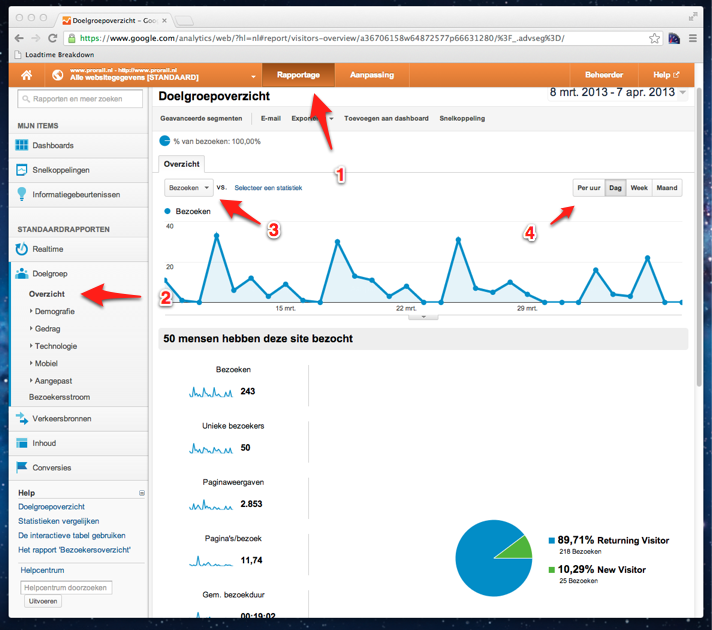
\includegraphics[width=\textwidth]{img/stats1.png}

Onderaan deze pagina zijn tevens een aantal kerncijfers te zien.

\clearpage
\subsubsection{Aantal bezoekers per doelgroep}

Binnen het doelgroep overzicht is ook het aantal bezoekers per doelgroep te vinden. Klik hiervoor op de knop "Geavanceerde segmenten". Er verschijnen nu twee kolommen. De linker bevat segmenten die standaard in GA aanwezig zijn. De rechter bevat aangepaste segmenten. Voor ProRail zijn de doelgroepen beschikbaar als een aangepast segment. Selecteer \'{e}\'{e}n of meerdere doelgroepen in deze lijst. Er kunnen maximaal 4 segmenten tegelijk worden getoond. Klik hierna op de knop "Toepassen". De geselecteerde doelgroepen verschijnen in een legenda en in de grafiek (ieder met een eigen kleur).
\\

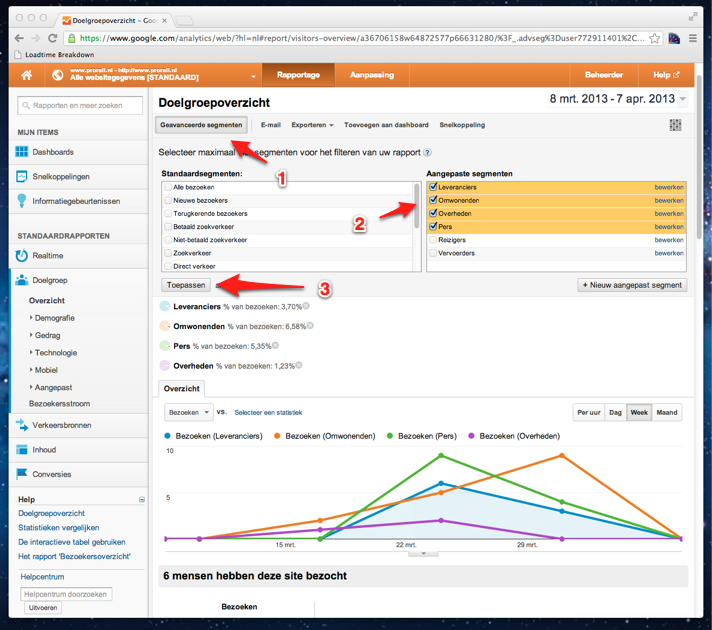
\includegraphics[width=\textwidth]{img/stats2.png}

\clearpage
\subsubsection{Klikgedrag / bezoekerspaden}
Onder \emph{Doelgroep} $\Rightarrow$ \emph{Bezoekersstroom} zijn de klikpaden van de bezoekers in te zien. Linksboven staat een dropdown waarin standaard "Alle bezoekers" staat (zie nummer 3 op de screenshot). Zo niet, klik hier dan op en klik op \emph{Alle bezoekers} onder \emph{Standaardsegmenten}.
\\

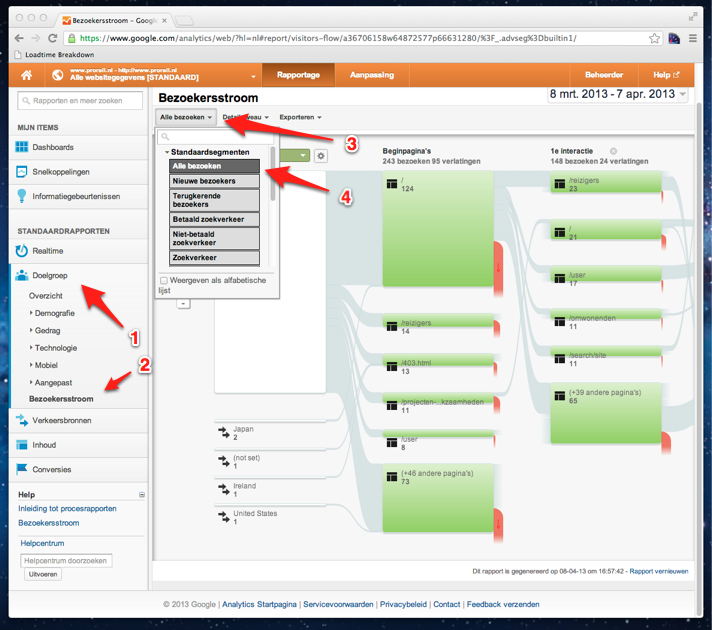
\includegraphics[width=\textwidth]{img/stats3.png}

\clearpage
\subsubsection{Lengte van bezoek}
De bezoeksduur is te vinden onder \emph{Doelgroep} $\Rightarrow$ \emph{Engagement}.
\\

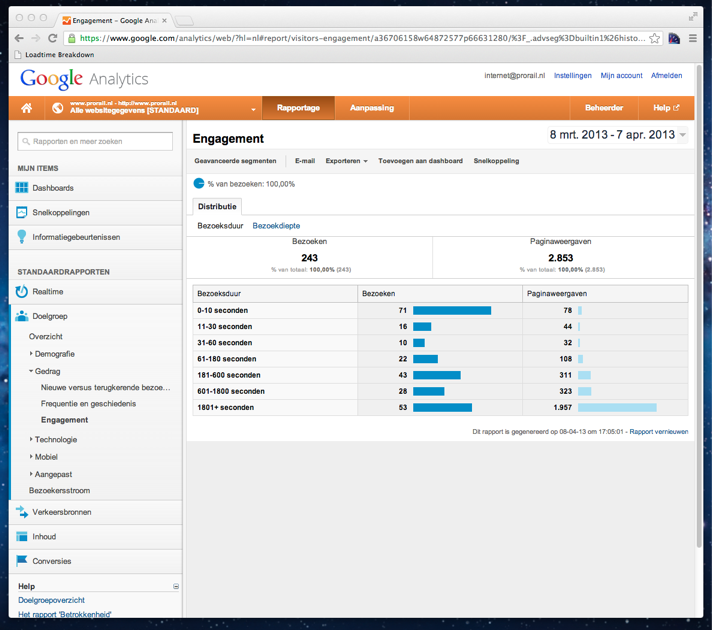
\includegraphics[width=\textwidth]{img/stats4.png}

\clearpage
\subsubsection{Exitpagina's}
Exitpagina's zijn te vinden onder \emph{Inhoud} $\Rightarrow$ \emph{Site-inhoud} $\Rightarrow$ \emph{Uitstappagina's}. De pagina's worden standaard in een lijst weergegeven. Het is ook mogelijk om deze in een cirkeldiagram of lijndiagram te tonen (zie 4 op de screenshot).
\\

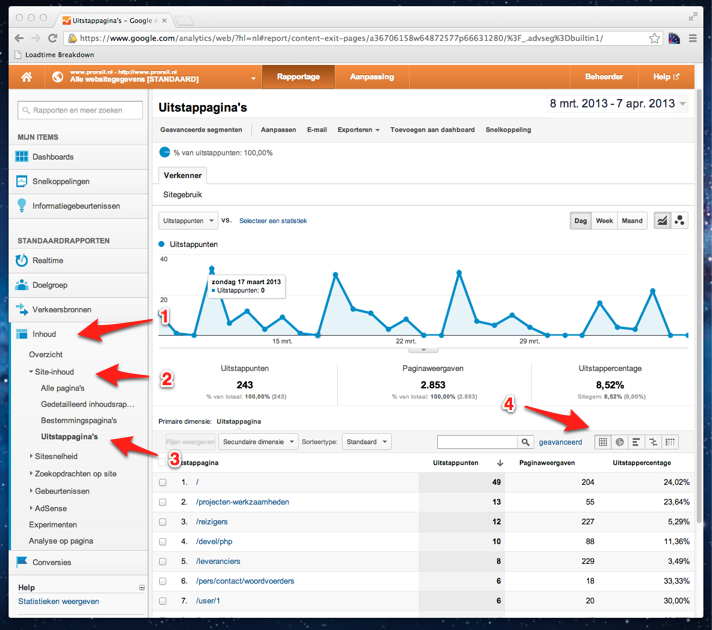
\includegraphics[width=\textwidth]{img/stats5.png}

\clearpage
\subsection{Rapportage per doelgroep}
\pvelist{ \pve{3.8.3.2} }
In GA is het mogelijk om alle eerder genoemde rapportages te filteren op \emph{segment}. Een segment in een deel van de bezoekers. Er zijn diverse mogelijkheden om de segmenten te defini\"{e}ren. Bij ProRail zijn al segmenten aangemaakt per doelgroep.

Door bovenin op de knop \emph{Geavanceerde segmenten} te klikken wordt een lijst getoond met alle beschikbare segmenten. Klik hiervoor op de knop "Geavanceerde segmenten". Er verschijnen nu twee kolommen. De linker bevat segmenten die standaard in GA aanwezig zijn. De rechter bevat aangepaste segmenten. Selecteer \'{e}\'{e}n of meerdere doelgroepen in deze lijst. Er kunnen maximaal 4 segmenten tegelijk worden getoond. Klik hierna op de knop "Toepassen".

De keuze voor segmenten blijft behouden wanneer naar een andere rapportage wordt geklikt. Om weer alle bezoekers te tonen zal gekozen moeten worden voor het segment "Alle bezoeken" in de linkerkolom (zie 2 op de screenshot).
\\

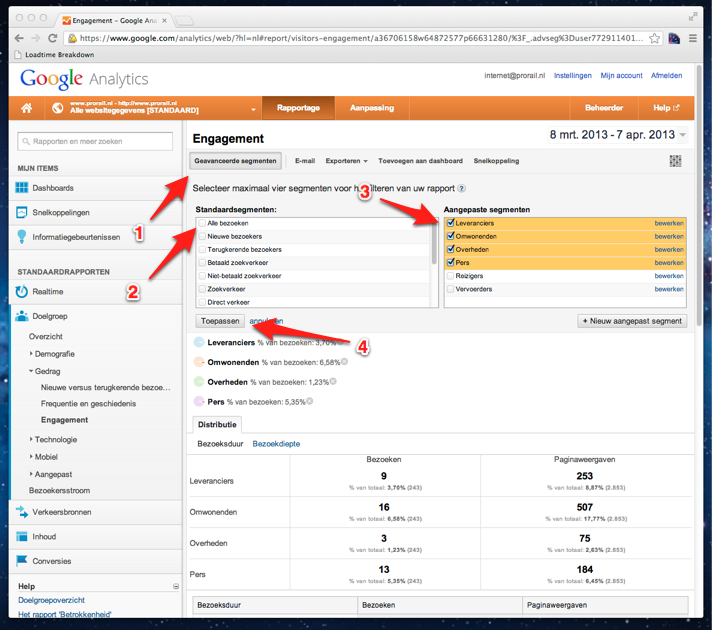
\includegraphics[width=\textwidth]{img/stats6.png}

\clearpage
\subsection{Veelgestelde vragen}
\pvelist{ \pve{3.8.3.3} }
De veelgestelde vragen staan verzameld met meer vragen per pagina. De statistieken zijn daarom niet te vinden tussen de pagina's, maar worden gemeten wanneer de vraag opengeklapt wordt. In GA heet dat een "gebeurtenis".


\subsubsection{Aantallen per vraag / categorie / doelgroep}
De veelgestelde vragen zijn te vinden onder \emph{Aanpassing} $\Rightarrow$ \emph{Aangepaste rapporten} $\Rightarrow$ \emph{Veelgestelde vragen}. Uitsplitsing naar segmenten (doelgroepen) is hier mogelijk via de knop \emph{Geavanceerde segmenten}.
\\

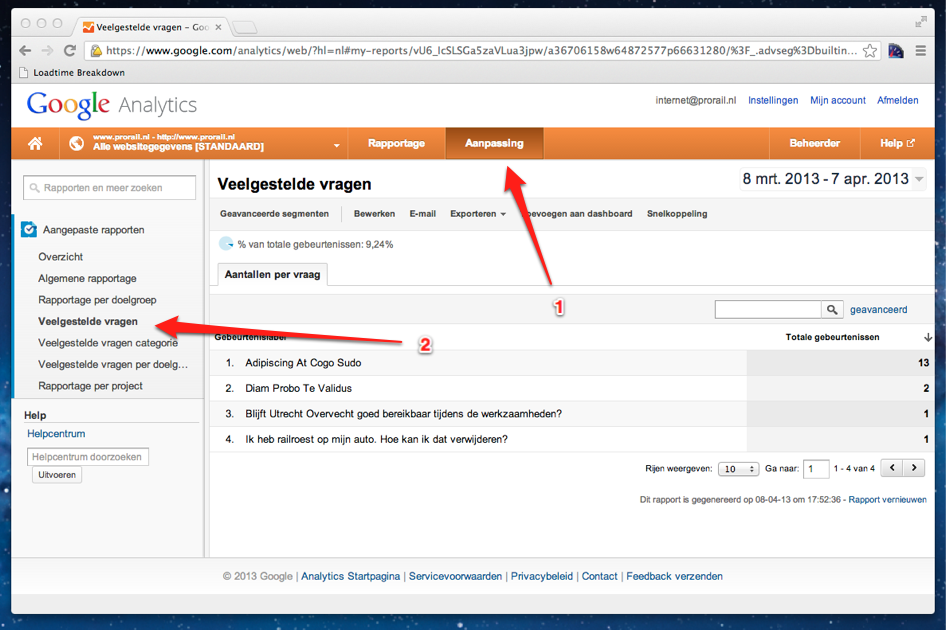
\includegraphics[width=\textwidth]{img/stats7.png}


\clearpage
\subsection{Zoekopdrachten}
\pvelist{ \pve{3.8.3.4} }

De zoekoprachten zijn te vinden onder \emph{Rapportage} $\Rightarrow$ \emph{Inhoud} $\Rightarrow$ \emph{Overzicht} $\Rightarrow$ \emph{Zoekopdrachten op de site} $\Rightarrow$ \emph{Zoektermen}. Uitsplitsing naar segmenten (doelgroepen) is hier mogelijk via de knop \emph{Geavanceerde segmenten}.

\subsection{Projectenrapportage}
\pvelist{ \pve{3.8.3.5} }
De eerder genoemde rapportages kunnen ook uitgesplitst worden per project. Hiervoor worden ook aangepaste segmenten gebruikt, gelijk aan de doelgroepen. De segmenten voor projecten zijn echter niet vooraf aangemaakt en moeten dus zelf toegevoegd worden. Klik hiervoor op \emph{Geavanceerde segmenten}. Dan verschijnen de twee kolommen met segmenten. Rechtsonder de tweede kolom staat een knop \emph{Nieuw aangepast segment}. Klik daarop om een nieuw segment voor een project toe te voegen.

Er verschijnt een formulier waarmee de definitie van het segment ingevoerd kan worden. In het groene vak moet aangegeven worden welke variabele we willen opnemen. Dit is "Vrije variabele (waarde 02)". Dit is de naam van de subsite. Let erop dat de waarde gebruikt wordt en niet de sleutel. Klik op de knop daarnaast en kies voor "Komt precies overeen". In het tekstvak ernaast kan de naam van de subsite opgegeven worden, bijv. "Hanzelijn". Kies hierna voor \emph{Segment opslaan}. Nu kan het segment op dezelfde manier worden gebruikt als bij de filtering op doelgroep. Het aanmaken van het segment is \'{e}\'{e}nmalig (per project).
\\

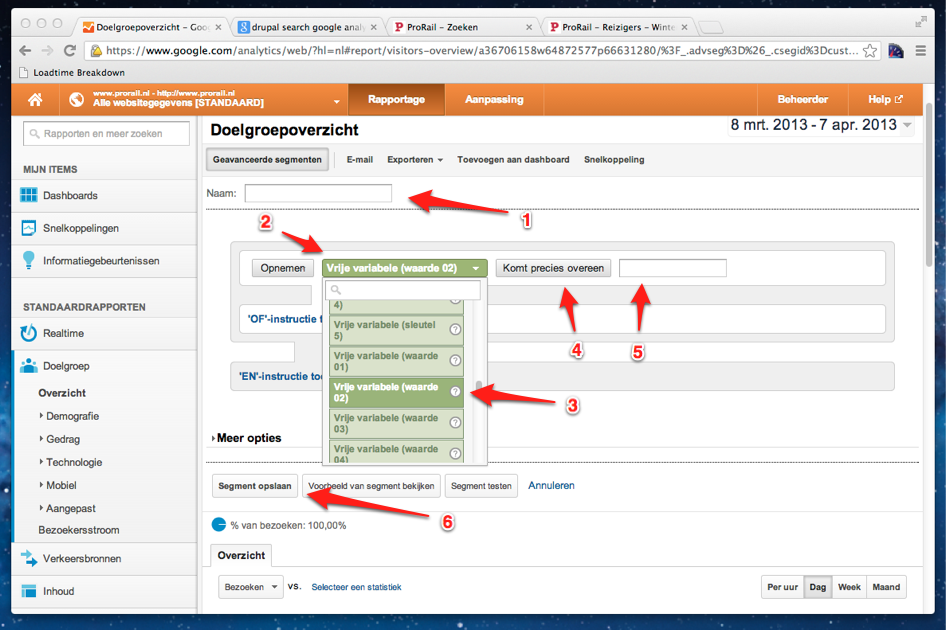
\includegraphics[width=\textwidth]{img/stats8.png}


\subsection{Paginarapportage}
\pvelist{ \pve{3.8.3.6} }
Per pagina kan onder andere het bezoekersaantal (views en uniek), de lengte van het bezoek en het klikpad worden ingezien. Ga hiervoor naar \emph{Rapportage} $\Rightarrow$ \emph{Inhoud} $\Rightarrow$ \emph{Overzicht} $\Rightarrow$ \emph{Site-inhoud} $\Rightarrow$ \emph{Alle pagina's}. In dit deel is een lijst te vinden van alle pagina's die zijn gemeten, standaard gesorteerd op meest bezocht. Klik op een pagina om meer informatie over deze specifieke pagina te zien. Hier is het aantal views te zien (2 in screenshot) en de gemiddelde tijd op de pagina (3 in screenshot).
\\

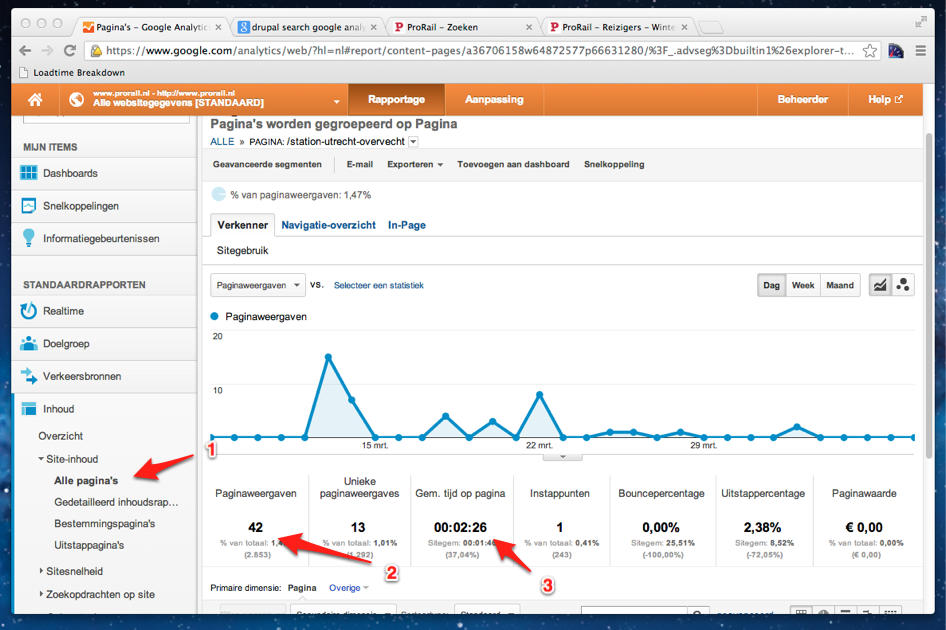
\includegraphics[width=\textwidth]{img/stats9.png}

Bovenaan de pagina kan worden gekozen voor \emph{Navigatie-overzicht}. Op de pagina daarachter kan worden ingezien vanaf welke pagina's men op deze pagina komt, en naar welke pagina men vanaf deze pagina navigeert. Hier worden ook de termen \emph{instappunten} en \emph{uitstappunten} gebruikt. Instappunten geeft het aantal bezoekers aan dat direct op deze pagina kwam zonder gebruik te maken van een link op een andere pagina (binnen deze website). Uitstappunten zijn het aantal bezoekers dat op deze pagina de site heeft verlaten
\\

\subsection{Downloadsrapportage}
Ga hiervoor naar Content $\Rightarrow$ Behavior Flow $\Rightarrow$ Events $\Rightarrow$ Top Events en klik dan op \emph{Downloads}. Daarna kan verder gefilterd worden op extensie (bijv. pdf) of kan op \emph{Event Label} worden geklikt om de lijst van bestanden te tonen.

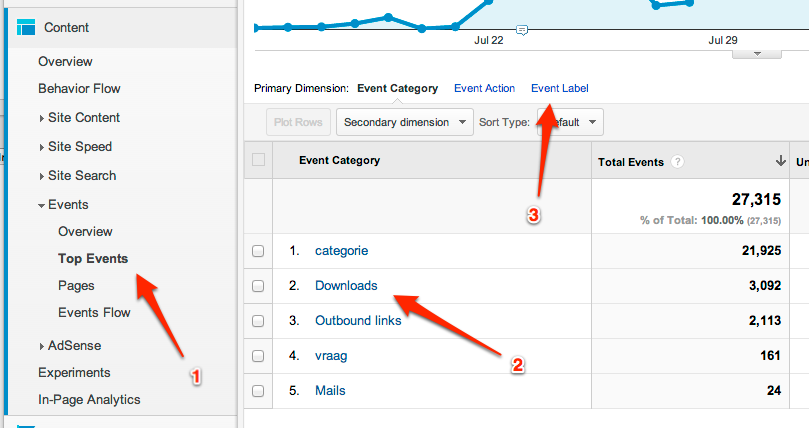
\includegraphics[width=\textwidth]{img/statsgadownloads.png}
